\subsection{Estados cuánticos y el término Qubit}
\subsection{Puertas lógicas clásicas y cuánticas}
\subsection{Operador de Hadamart}
\subsubsection{Transformada de Fourier clásica y cuántica}
\subsection{Algoritmo de Shor}
\subsubsection{Periodo de la función $a^x mod N$}
Se tiene la función \begin{equation}
    f(x)=a^x mod N
    \label{eq:axmodn}
\end{equation}
donde $a$ y $N$ son enteros positivos tal que $a<N$ y que no tienen ningún factor en común. El periodo (o el orden r), es el valor más pequeño 
diferente de cero tal que:
\begin{equation}
    a^r mod N =1
    \label{eq:condicionr}
\end{equation}
Usando como ejemplos $a=3$ y $N=35$, se tiene el siguiente periodo:
\begin{figure}[H]
    \centering
    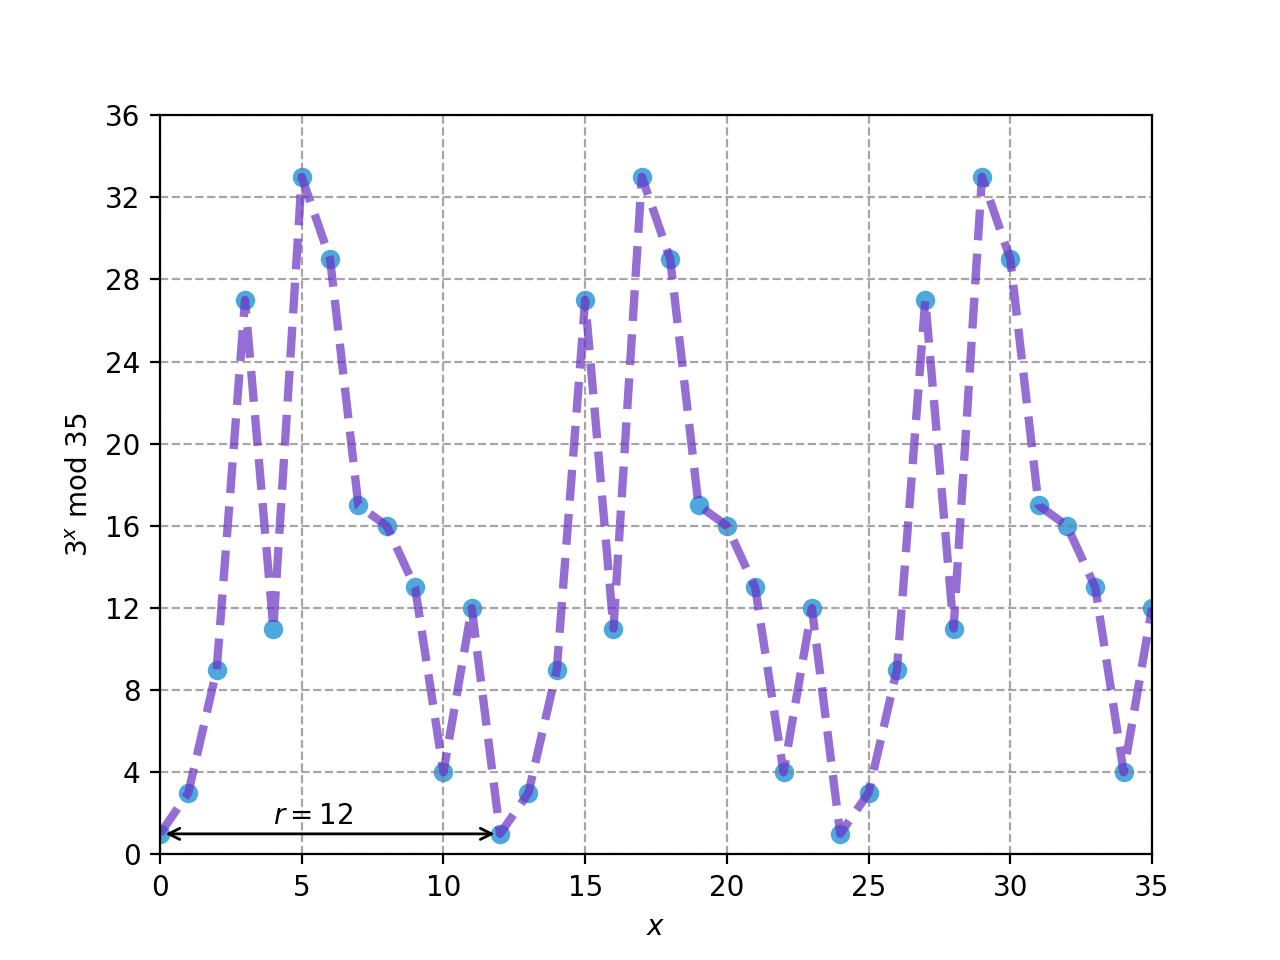
\includegraphics[scale=0.65]{../Graphics/period.png}
    \caption{Periodo de la función \ref{eq:axmodn} para visualizar la condición \ref{eq:condicionr}}
    \label{fig:condicionr}
\end{figure}
\subsection{Implementación con Qiskit}